% !TEX encoding = UTF-8 Unicode
\documentclass[a4paper]{article}

\usepackage{color}
\usepackage[obeyspaces]{url}
\usepackage[T1]{fontenc} % enable Cyrillic fonts
\usepackage[utf8]{inputenc} % make weird characters work
\usepackage{graphicx}
\usepackage[margin=1.0in]{geometry}
\usepackage[table]{xcolor}
\usepackage{tocloft}
\usepackage{float}
\addtolength{\cftsecnumwidth}{10pt}
\usepackage{wasysym}


\usepackage[english,serbian]{babel}
%\usepackage[english,serbianc]{babel} 

\PassOptionsToPackage{obeyspaces}{url}
\usepackage[unicode]{hyperref}
\hypersetup{colorlinks,citecolor=green,filecolor=green,linkcolor=blue,urlcolor=blue}

\usepackage{listings}
\renewcommand\lstlistingname{Kod}
\renewcommand\lstlistlistingname{Kodovi}

\definecolor{mygreen}{rgb}{0,0.6,0}
\definecolor{mygray}{rgb}{0.5,0.5,0.5}
\definecolor{mymauve}{rgb}{0.58,0,0.82}

\lstset{
  backgroundcolor=\color{white},   % choose the background color; you must add \usepackage{color} or \usepackage{xcolor}; should come as last argument
  basicstyle=\scriptsize\ttfamily,        % the size of the fonts that are used for the code
  breakatwhitespace=false,         % sets if automatic breaks should only happen at whitespace
  breaklines=true,                 % sets automatic line breaking
  captionpos=b,                    % sets the caption-position to bottom
  commentstyle=\color{mygreen},    % comment style
  deletekeywords={...},            % if you want to delete keywords from the given language
  escapeinside={\%*}{*)},          % if you want to add LaTeX within your code
  extendedchars=true,              % lets you use non-ASCII characters; for 8-bits encodings only, does not work with UTF-8
  firstnumber=1,                   % start line enumeration with line 1000
  frame=single,	                   % adds a frame around the code
  keepspaces=true,                 % keeps spaces in text, useful for keeping indentation of code (possibly needs columns=flexible)
  keywordstyle=\color{blue},       % keyword style
  language=Python,                 % the language of the code
  morekeywords={*,...},            % if you want to add more keywords to the set
  numbers=left,                    % where to put the line-numbers; possible values are (none, left, right)
  numbersep=5pt,                   % how far the line-numbers are from the code
  numberstyle=\tiny\color{mygray}, % the style that is used for the line-numbers
  rulecolor=\color{black},         % if not set, the frame-color may be changed on line-breaks within not-black text (e.g. comments (green here))
  showspaces=false,                % show spaces everywhere adding particular underscores; it overrides 'showstringspaces'
  showstringspaces=false,          % underline spaces within strings only
  showtabs=false,                  % show tabs within strings adding particular underscores
  stepnumber=2,                    % the step between two line-numbers. If it's 1, each line will be numbered
  stringstyle=\color{mymauve},     % string literal style
  tabsize=2,	                     % sets default tabsize to 2 spaces
  title=\lstname                   % show the filename of files included with \lstinputlisting; also try caption instead of title
}

\usepackage{enumitem}
\newlist{legal}{enumerate}{10}
\setlist[legal]{label*=\arabic*.}

\begin{document}

\title{Informacioni sistem pozorišta\\ \small{Seminarski rad u okviru kursa\\Informacioni sistemi\\ Matematički fakultet}}

\author{
Katarina Savičić 1086/2020\\
Dragana Milić 1042/2019\\
Nikola Vuković 1090/2020\\
Ognjen Milinković 1008/2020\\
Momir Adžemović 1005/2020
}

\date{1.~april 2020.}

\maketitle

\abstract

Ovo je sažetak.

\newpage

\tableofcontents

\newpage

\section{Uvod}
Ovaj rad se bavi modeliranjem najvažnijih procesa u radu jednog pozorišta, gde se akcenat
stavlja na proces produkcije predstave. Proces predstave se sastoji iz dva glavna 
dela:\cite{hamilton_theatre_producing_the_drama}
\begin{itemize}
  \item priprema i izvođenje
  \item tehnički deo
\end{itemize}

\section{Slučajevi upotrebe}

\subsection{Organizacija predstave}
Proces organizacije predstave počinje prijavom koju popunjava i podnosi organizator. Predstavu sa statusom "prijavljena" mora da odobri supervizor pozorišta. Kada se prijavljena predstava odobri, onda predstava prelazi u stanje "u pripremi". 

Organizator predstave je zadužen za ceo proces formiranja predstave od njene prijave do realizacije, dok supervizor izvršava administrativne zadatke vezane za pozorište. Neophodno je da organizator konstantno ima uvid u stanje svake predstave za koji je on zadužen. 

\begin{figure}[H]
  \begin{center}
      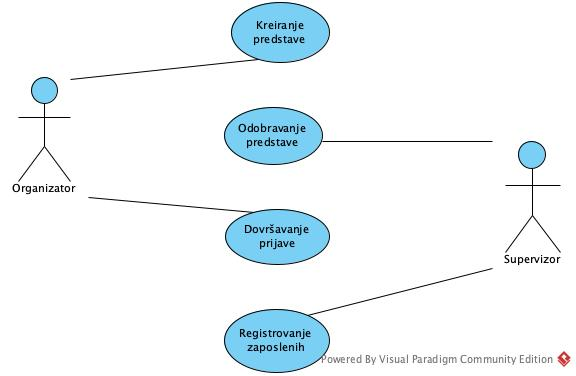
\includegraphics[width=100mm,height=60mm]{../diagrams/usecase_organizacija_predstave.jpg}
  \end{center}
  \caption{Organizacija predstave}
  \label{usecase_prodaja_karata}
\end{figure}

\subsubsection{Kreiranje predstave} \label{Kreiranje predstave}
\noindent\textbf{Kratak opis:} Da bi se predstava održala, organizator mora da je kreira u informacionom sistemu. 

\noindent\textbf{Učesnici:} Zaposleni koji je organizator predstave

\noindent\textbf{Preduslovi:}
  \begin{itemize}
    \item Postoji zaposleni koji je organizator predstave.
    \item Postoji scenario za predstavu.
    \item Organizator je ugovorio izvođenje predstave sa rediteljem.
    \item Reditelj je odredio glumce.
    \item Procenjen je budžet koji uključuje platu glumaca tokom pripreme i izvođenja, dužinu pripreme, i elemente scene.
    \item Reditelj i glumci su registrovani u sistemu kao zaposleni.
  \end{itemize}

\noindent\textbf{Postuslovi:} 
  \begin{itemize}
    \item Kreirana predstava je sačuvana u sistemu sa statusom "prijavljena".
    \item Organizator može da vidi prijavljenu predstavu kada je prijavljen na sistem.
  \end{itemize}

\noindent\textbf{Osnovni tok:}
  \begin{legal}
    \item Organizator u sistemu otvara stranu za kreiranje predstave.
    \item Organizator unosi u formu potrebne informacije, uključujući ime i opis predstave, reditelja, glumce i uloge. 
    \item Organizator evidentira prijavu predstave u sistem klikom na "Pošalji prijavu". 
    \item Supervizor se obaveštava mailom o prijavljenoj predstavi.
  \end{legal}

\noindent\textbf{Alternativni tokovi:} 
\begin{itemize}
  \item \textbf{A1. Informacije o prijavi su nepotpune} 
      \begin{legal}
        \item Organizator u koraku 2. ne unosi sve informacije, ili nije siguran da li su informacije finalne. 
        \item Organizator čuva predstavu sa statusom "nedovršena" klikom na "Sačuvaj nedovršenu prijavu".
      \end{legal}
  \item \textbf{A2. Neki od uključenih zaposlenih nije evidentiran u sistemu} 
      \begin{legal}
        \item Organizator ne može da dovrši korak 2 jer jedan od zaposlenih nije evidentiran u sistemu, pa čuva nedovršenu prijavu (Alternativni tok A1)
        \item Supervizor evidentira zaposlenog u sistemu procesom opisanim u \ref{Registrovanje zaposlenih}.
        \item Organizator nastavlja proces kroz \ref{Dovršavanje prijave}
      \end{legal}
\end{itemize}

\noindent\textbf{Dodatne informacije:} Podrazumeva se da je predstava ugovorena drugim putevima - nizom mailova, telefonskih razgovora i sastanaka. Zbog komplikovane prirode međuljudskih veza u ovoj sferi, informacioni sistem se bavi isključivo ugovorenom predstavom. 

\subsubsection{Odobravanje predstave}
\noindent\textbf{Kratak opis:} Kada je predstava prijavljena, supervizor pregleda informacije, uzimajući u obzir aktuelni i budući repertoar i interesovanje publike za isti, kao i budžet pozorišta, i odobrava predstavu. 

\noindent\textbf{Učesnici:} Supervizor pozorišta.

\noindent\textbf{Preduslovi:}
  \begin{itemize}
    \item Određena predstava je evidentirana u sistemu kao "prijavljena".
  \end{itemize}

\noindent\textbf{Postuslovi:} 
  \begin{itemize}
    \item Predstava koja je bila evidentirana kao "prijavljena" je evidentirana kao "u pripremi"
    \item Organizator može da vidi odgovarajući status predstave nakon prijave na sistem.
    \item Organizator može da rezerviše sale za probu i održavanje predstave. 
  \end{itemize}

\noindent\textbf{Osnovni tok:}
  \begin{legal}
    \item Supervizor pretražuje predstave sa statusom "prijavljena".
    \item Supervizor otvara stranu za prikaz informacija o određenoj prijavljenoj predstavi. 
    \item Nakon analize informacija, supervizor odobrava predstavu. 
    \item Organizator se obaveštava mailom o odobrenju. 
  \end{legal}

\noindent\textbf{Alternativni tokovi:} 
\begin{itemize}
  \item \textbf{A1. Predstava je odbijena} 
      \begin{legal}
        \item Supervizor u 3. koraku odbija prijavu predstave uz obrazloženje.
        \item Organizator se obaveštava mailom o odbijanju uz obrazloženje. 
      \end{legal}
\end{itemize}


\subsubsection{Dovršavanje prijave} \label{Dovršavanje prijave}
\noindent\textbf{Kratak opis:} U slučaju da je organizator sačuvao prijavu kao nedovršenu, može da je izmeni ili dopuni, i konačno pošalje. 

\noindent\textbf{Učesnici:} Organizator predstave

\noindent\textbf{Preduslovi:}
  \begin{itemize}
    \item Organizator je započeo prijavu predstave i sačuvao je kao nedovršenu.
    \item Organizator može da vidi nedovršenu predstavu nakon prijave na sistem.
    \item Svi preduslovi slučaja \ref{Kreiranje predstave}.
  \end{itemize}

\noindent\textbf{Postuslovi:} 
  \begin{itemize}
    \item Predstava koja je bila evidentirana kao "nedovršena" je sada evidentirana kao "prijavljena".
    \item Svi postuslovi slučaja \ref{Kreiranje predstave}.
  \end{itemize}

\noindent\textbf{Osnovni tok:}
  \begin{legal}
    \item Organizator pretražuje nedovršene prijave.
    \item Organizator otvara određenu nedovšenu prijavu. 
    \item Organizator dopunjava, odnosno menja željene informacije.
    \item Organizator evidentira prijavu predstave u sistem klikom na "Pošalji prijavu". 
    \item Supervizor se obaveštava mailom o prijavljenoj predstavi.
  \end{legal}

\noindent\textbf{Alternativni tokovi:} 
\begin{itemize}
  \item \textbf{A1. Informacije o prijavi su nepotpune} 
      \begin{legal}
        \item Organizator u koraku 2. ne unosi sve informacije, ili nije siguran da li su informacije finalne. 
        \item Organizator čuva predstavu sa statusom "nedovršena" klikom na "Sačuvaj nedovršenu prijavu".
      \end{legal}
\end{itemize}


\subsubsection{Registrovanje zaposlenih} \label{Registrovanje zaposlenih}
\noindent\textbf{Kratak opis:} Da bi zaposleni bili uključeni u predstavu, moraju biti registrovani u sistemu. Supervizor po sklapanju ugovora o radu sa zaposlenima unosi njihove informacije u sistem

\noindent\textbf{Učesnici:} Supervizor

\noindent\textbf{Preduslovi:}
  \begin{itemize}
    \item Pozorište je sklopilo ugovor o radu sa osobom A.
  \end{itemize}

\noindent\textbf{Postuslovi:} 
  \begin{itemize}
    \item Osoba A je eveidentirana kao zaposleni u sistemu.
    \item Osoba A može da se prijavi na sistem.
  \end{itemize}

\noindent\textbf{Osnovni tok:}
  \begin{legal}
    \item Supervizor otvara formu za evidentiranje zaposlenog.
    \item Supervizor popunjava formu, unoseći sve potrebne informacije uključujući Ime, Prezime, JMBG i email adresu. 
    \item Zaposleni je obavešten o kreiranom profilu putem emaila. 
    \item Zaposleni klikom na link u emailu koji mu je stigao odlazi na stranicu gde kreira šifru za svoj nalog i potvrđuje registraciju.  
  \end{legal}

\noindent\textbf{Alternativni tokovi:} 
\begin{itemize}
  \item \textbf{A1. Zaposleni ne potvrđuje registraciju} 
      \begin{legal}
        \item Zaposleni nije ispunio 4. korak. Zaposleni ne može da se prijavi na sistem ali može da bude uključen u prijavu predstave. 
      \end{legal}
\end{itemize}



% --------------------------------------------------------------------------------------------------

\subsection{Rezervacija pozorišnih sala}
\begin{enumerate}
  \item \textbf{Kratak opis:} Organizator predstave u pripremi treba da rezerviše salu za probu ili konkretnu predstavu. Dakle, treba omogućiti uvid u slobodne sale, 
        kao i rezervacije unapred. Ukoliko dodje do promene termina predstave ili probe, potrebno je promeniti i termin za salu. Organizator ima mogućnost promene sale ukoliko je druga sala slobodna za dati termin. 
\end{enumerate}
\subsubsection{Prijavljivanje sale}
\noindent\textbf{Kratak opis:} Kada je predstava odobrena, organizator rezerviše salu za određeni datum i vreme za održavanja predstave ili probe. 

\noindent\textbf{Učesnici:} Organizator pozorišta.

\noindent\textbf{Preduslovi:}
  \begin{itemize}
    \item Određena predstava je evidentirana u sistemu kao "odobrena".
  \end{itemize}

\noindent\textbf{Postuslovi:} 
  \begin{itemize}
    \item Sala za održavanje predstave ili probe je rezervisana za određeni datum i vreme
    \item Organizator i glumci imaju uvid u kojoj se sali održava predstava ili proba  nakon prijave na sistem.
  \end{itemize}

\noindent\textbf{Osnovni tok:}
  \begin{legal}
  \item Organizator unosi podatke za prijavljivanje na sistem.
    \item Sistem vrši verifikaciju i prikazuje organizatoru listu predstava za koje je zadužen.
    \item Organizator bira predstavu sa statusom "odobrena" kojoj želi da dodeli salu .
    \item Sistem prikazuje informacije o predstavi.
    \item Organizator unosi datum i vreme održavanja predstave
    \item Organizator unosi dužinu trajanja predstave
    \item Sistem prikazuje slobodne sale za dati termin.
    \item Organizator dodeljuje slobodnu salu datoj predstavi za određeni termin.
    \item Sistem ažurira bazu podataka.
    \item Glumci se obaveštavaju mailom o sali za održavanje predstave ili probe. 
  \end{legal}

\noindent\textbf{Alternativni tokovi:} 
\begin{itemize}
 \item \textbf{A1. Neuspelo prijavljivanje} 
      \begin{legal}
        \item Sistem prikazuje poruku o grešci pri prijavljivanju..
        \item Proces se nastavlja u \textbf{koraku 1}.
      \end{legal}
  \item \textbf{A7. Sve sale su zauzete za odabrani termin} 
    \begin{legal}
      \item Sistem prikazuje poruku da su sve sale zauzete za dati termin.
      \item Proces se nastavlja u \textbf{koraku 5}.
    \end{legal}
\end{itemize}
\subsubsection{Odjavljivanje sale}
\noindent\textbf{Kratak opis:} Predstava je odložena i organizator odjavljuje datu salu

\noindent\textbf{Učesnici:} Organizator pozorišta.

\noindent\textbf{Preduslovi:}
  \begin{itemize}
    \item Predstavi je dodeljena sala
  \end{itemize}

\noindent\textbf{Postuslovi:} 
  \begin{itemize}
    \item Sala je oslobođena za dati termin
    \item Predstavi nije dodeljena nijedna sala
  \end{itemize}

\noindent\textbf{Osnovni tok:}
  \begin{legal}
  \item Organizator unosi podatke za prijavljivanje na sistem.
    \item Sistem vrši verifikaciju i prikazuje organizatoru listu predstava za koje je zadužen.
    \item Organizator bira predstavu kojoj je dodeljena sala .
    \item Sistem prikazuje informacije o predstavi.
    \item Organizator odjavljuje salu za dati termin
    \item Sistem ažurira bazu podataka.
    \item Glumci se obaveštavaju mailom o oslobođenom terminu za datu salu
  \end{legal}

\noindent\textbf{Alternativni tokovi:} 
\begin{itemize}
 \item \textbf{A1. Neuspelo prijavljivanje} 
      \begin{legal}
        \item Sistem prikazuje poruku o grešci pri prijavljivanju.
        \item Proces se nastavlja u \textbf{koraku 1}.
      \end{legal}
  
\end{itemize}


\subsubsection{Promena sale}
\noindent\textbf{Kratak opis:} Organizator može da promeni salu za održavanje predstave ukoliko je zbog velikog interesovanja gledalaca potrebna sala sa većim kapacitetom

\noindent\textbf{Učesnici:} Organizator pozorišta.

\noindent\textbf{Preduslovi:}
  \begin{itemize}
    \item Predstava ili probi je dodeljena nova sala
  \end{itemize}

\noindent\textbf{Postuslovi:} 
  \begin{itemize}
    \item Predstavi ili probi je promenjena  sala za održavanje
    \item Prvobitno izabrana sala je oslobođena za dati termin
  \end{itemize}

\noindent\textbf{Osnovni tok:}
  \begin{legal}
  \item Organizator unosi podatke za prijavljivanje na sistem.
    \item Sistem vrši verifikaciju i prikazuje organizatoru listu predstava za koje je zadužen.
    \item Organizator bira predstavu kojoj je dodeljena sala .
    \item Sistem prikazuje informacije o predstavi.
    \item Sistem prikazuje slobodne sale za dati termin.
    \item Organizator dodeljuje slobodnu salu datoj predstavi za određeni termin.
     \item Sistem ažurira bazu podataka.
    \item Glumci se obaveštavaju mailom o promeni sale za održavanje predstave ili probe
  \end{legal}

\noindent\textbf{Alternativni tokovi:} 
\begin{itemize}
 \item \textbf{A1. Neuspelo prijavljivanje} 
      \begin{legal}
        \item Sistem prikazuje poruku o grešci pri prijavljivanju..
        \item Proces se nastavlja u \textbf{koraku 1}.
      \end{legal}
       \item \textbf{A5. Sve sale su zauzete za odabrani termin} 
    \begin{legal}
      \item Sistem prikazuje poruku da su sve sale zauzete za dati termin.
      \item Slučaj upotrebe se ovde završava
    \end{legal}
\end{itemize}

\subsection{Održavanje predstave}
  \item \textbf{Kratak opis:} Supervizor treba da napravi repertoar po kome se odrzavaju predstave, kao i da nedelju dana unapred proverava da li je došlo do promene (otkazivanja predstave), dok šef razvodnika treba da napravi raspored rada razvodnika u zavisnosti od repertoara. 
  
  \begin{figure}[H]
  \begin{center}
      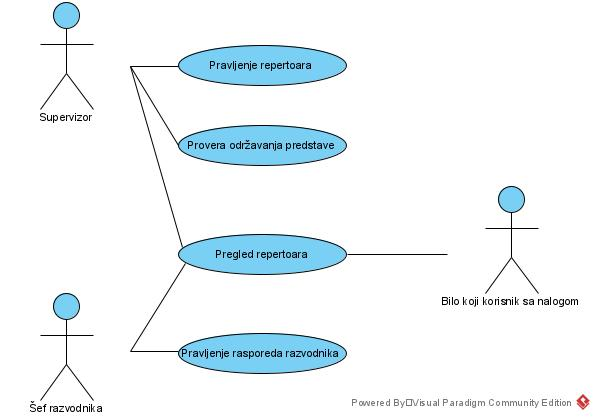
\includegraphics[width=100mm,height=60mm]{../diagrams/usecase_odrzavanje_predstave.jpg}
  \end{center}
  \caption{Održavanje predstave}
  \label{usecase_prodaja_karata}
\end{figure}


\subsubsection{Pravljenje repertoara} 
\noindent\textbf{Kratak opis:} Supervizor treba da napravi repertoar za narednih mesec dana, imajući u vidu sve predstave koje su spremne za izvođenje.

\noindent\textbf{Učesnici:} Supervizor pozorišta.

\noindent\textbf{Preduslovi:}
  \begin{itemize}
    \item Postoji zaposleni koji je zadužen za repertoar, i to je u ovom slučaju supervizor.
    \item Postoji spisak svih predstava koje se izvode sledećeg meseca.
    \item Supervizor ima pristup spisku predstava i poznato je trajanje i sala u kojoj se izvodi svaka predstava.
  \end{itemize}

\noindent\textbf{Postuslovi:} 
  \begin{itemize}
    \item Napravljen je repertoar.
    \item Repertoar može da pogleda bilo koji korisnik sistema koji ima pristup internetu.
  \end{itemize}

\noindent\textbf{Osnovni tok:}
  \begin{legal}
    \item Supervizor otvara formu za evidentiranje zaposlenog.
    \item Supervizor pristupa spisku predstava koje treba da se nađu na repertoaru.
    \item Supervizor sastavlja repertoar, tako što za svaki dan bira koja će se predstava kad i gde održavati.  
  \end{legal}

\noindent\textbf{Alternativni tokovi:} 
\begin{itemize}
  \item \textbf{A1. Nije moguće održati predstavu zbog gostovanja} 
      \begin{legal}
        \item Za određeni dan nije moguće realizovati korak 2.
        \item Umesto predstave tog dana, na repertoaru će se naći gostovanje.
      \end{legal}
\end{itemize}

\subsubsection{Pravljenje rasporeda razvodnika} 
\noindent\textbf{Kratak opis:} Šef razvodnika treba da napravi raspored rada razvodnika u zavisnosti od repertoara.

\noindent\textbf{Učesnici:} Šef razvodnika.

\noindent\textbf{Preduslovi:}
  \begin{itemize}
    \item Poznat je repertoar.
    \item Poznato je koji razvodnici rade sledećeg meseca.
    \item Šef razvodnika ima pristup sistemu.
  \end{itemize}

\noindent\textbf{Postuslovi:} 
  \begin{itemize}
    \item Poznat je raspored razvodnika za svaki dan repertoara.
    \item Bilo koji razvodnik može da pogleda raspored rada razvodnika za tekući mesec.
  \end{itemize}

\noindent\textbf{Osnovni tok:}
  \begin{legal}
    \item Šef razvodnika pristupa sistemu.
    \item Šef razvodnika pregleda repertoar za svaki dan posebno.
    \item Šef razvodnika određuje koji će razvodnici biti u kojoj sali za svaki dan koji pregledaju.  
  \end{legal}


\subsubsection{Provera održavanja predstave} 
\noindent\textbf{Kratak opis:} Supervizor svakog dana proverava predstave koje suna repertoaru nedelju istog dana sledeće nedelje, za slučaj da je neka otkazana.

\noindent\textbf{Učesnici:} Supervizor pozorišta.

\noindent\textbf{Preduslovi:}
  \begin{itemize}
    \item Poznat je repertoar.
    \item Supervizor ima pristup sistemu.
  \end{itemize}

\noindent\textbf{Postuslovi:} 
  \begin{itemize}
    \item Vidljive su izmene u repertoaru.
  \end{itemize}

\noindent\textbf{Osnovni tok:}
  \begin{legal}
    \item Supervizor pristupa sistemu.
    \item Supervizor proverava da li postoji neki problem sa predstavama koje se odr.avaju nedelju dana od dana kada vrši proveru.
    \item Ukoliko postoji problem oko izvođenja predstave (predstava mora da bude otkazana), supervizor uklanja predstavu sa repertoara.
    \item Supervizor obaveštava blagajnu da je predstava otkazana, kako bi rešili probleme sa kartama za otkazanu predstavu.
  \end{legal}


\subsubsection{Pregled repertoara} 
\noindent\textbf{Kratak opis:} Bilo koji korisnik ima pristup repertoaru.

\noindent\textbf{Učesnici:} Korisnik servisa.

\noindent\textbf{Preduslovi:}
  \begin{itemize}
    \item Poznat je repertoar.
    \item Korisnik ima pristup sistemu.
  \end{itemize}

\noindent\textbf{Postuslovi:} 
  \begin{itemize}
    \item Korisnik je upoznat sa repertoarom.
  \end{itemize}

\noindent\textbf{Osnovni tok:}
  \begin{legal}
    \item Korisnik pristupa sistemu.
    \item Korisnik pregleda repertoar.
  \end{legal}



\newpage
\subsection{Prodaja karata}
Prodaja karata je proces koji sledi nakon što je određen datum, rezervisana sala i dodeljene uloge
zaposlenim. Tada je moguće preciznije odrediti potreban budžet za dalju realizaciju predstave, pa
samim tim i minimalni broj kupljenih karata za izvođenje. Na osnovu rezervisane sale (i potencijalno još 
nekih drugih faktora, kao što je epidemija ili slično), određuje se broj karata za prodaju. Gledaoci 
(klijenti) predstave mogu da kupe ili rezervišu kartu za pozorište preko veb stranice pozorišta. 
Takođe, klijenti mogu da kupe rezervisanu kartu ili nerezervisanu kartu ako nisu rasprodate na blagajni.
Klijent ima pravo da zatraži povraćaj novca za kupljenu kartu, a slučaju da se cela predstava otkaže,
potrebno je uz potvrdu organizatora da se izvrši povraćaj novca svim klijentima.

\begin{figure}[H]
  \begin{center}
      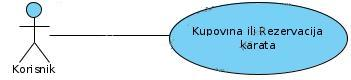
\includegraphics[width=100mm,height=60mm]{../diagrams/usecase_prodaja_karata.jpg}
  \end{center}
  \caption{Prodaja karata}
  \label{usecase_prodaja_karata}
\end{figure}

\subsubsection{Definisanje broja karata za predstavu}
\noindent\textbf{Kratak opis:} Organizator predstave može da definiše broj karata na osnovu rezervisane
sale za izvođenje predstave. Nakon definisanja se ažurira repertoar na stranici pozorište.\\

\noindent\textbf{Učesnici:} Organizator predstave.\\

\noindent\textbf{Preduslovi:}
  \begin{itemize}
    \item Predstava je zakazana određenog datuma.
    \item Rezervisana je određena sala za predstavu.
    \item Dodeljene su sve uloge (tehničke i umetničke) za realizaciju predstave .
    \item Određen je potreban budžet za realizaciju.
    \item Organizator je zaduđen za barem jednu predstavu.
  \end{itemize}

\noindent\textbf{Postuslovi:} 
  \begin{itemize}
    \item Ažuriran je repertoar tj. dodata je nova predstava sa kratkim opisom i datumom izvođenja.
    \item Ažuriran je status predstave u bazi podataka.
    \item Korisnici su u mogućnosti da rezervišu ili kupe kartu za tu predstavu.
  \end{itemize}

\noindent\textbf{Osnovni tok:}
  \begin{legal}
    \item Organizator unosi podatke za prijavljivanje na sistem.
    \item Sistem vrši verifikaciju i prikazuje organizatoru listu predstava za koje je on zadužen.
    \item Organizator bira predstavu koju želi da ažurira.
    \item Sistem prikazuje informacije o predstavi.
    \item Organizator unosi broj karata za prodaju i opciono dodaje napomenu.
    \item Sistem proverava unete podatke.
    \item Sistem ažurira bazu podataka.
  \end{legal}

\noindent\textbf{Alternativni tokovi:} 
\begin{itemize}
  \item \textbf{A1. Neuspelo prijavljivanje (korak 1)} 
      \begin{legal}
        \item Sistem prikazuje poruku o grešci pri prijavljivanju..
        \item Proces se nastavlja u \textbf{koraku 1}.
      \end{legal}
  \item \textbf{A2. Podaci o broju karata nisu validni (korak 6)} 
    \begin{legal}
      \item Sistem prikazuje poruku o grešci.
      \item Proces se nastavlja u \textbf{koraku 5}.
    \end{legal}
\end{itemize}

\noindent\textbf{Dodatne informacije:} 
  \begin{itemize}
    \item Postoji period osvežavanja repertoara na stranici na osnovu
          sadržaja baze podataka. 
    \item Sistem automatki popunjava vrednost polja za broj karata sa podrazumevanom
          vrednošću koja odgovara broju mesta u sali u kojoj je predstava zakazana.
  \end{itemize}

\subsubsection{Registracija i prijavljivanje na stranicu pozorišta}
  \textbf{Napomena:} Registracija i prijavljivanje je potrebno izdvojiti u poseban slučaj upotrebe.

\subsubsection{Onlajn kupovina karata i rezervacija}

\noindent\textbf{Kratak opis:} Informacioni sistem nudi pregled repertoara korisnicima. 
        Svako može da kupi kartu za određenu predstavu ako postoji slobodno mesto.
        Alternativa je da se vrši rezervacija karte koja se kasnije može da kupi u blagajni.\\

\noindent\textbf{Učesnici:} Registrovan korisnik koji želi da kupi ili rezerviše kartu.\\

\noindent\textbf{Preduslovi:} 
  \begin{itemize}
    \item Korisnik mora da bude registrovan sa odgovarajućim mejlom. 
    \item Korisnik mora da ima pristup internetu.
    \item Sistem mora da bude u funkciji.
    \item Sistem mora da bude pouzdan. 
    \item Mora da postoji barem jedno slobodno mesto za željenu predstavu, a samim tim mora da 
          postoji barem jedna aktivna predstava. 
    \item Ukoliko korisnik želi da kupi kartu, mora da ima karticu za online plaćanje (ili 
          alternativu neku).
  \end{itemize}
  
\noindent\textbf{Postuslovi:} 
  \begin{itemize}
    \item Korisnik je dobio potvrdu na mejl sa kodom kupljenje ili rezervisane karte.
    \item Ako je korisnik kupio kartu, onda je takođe dobio mejl sa informacijama računa.
    \item Baza je ažurirana tj. broj karata za predstavu je umanjen za broj kupljenih karata.
  \end{itemize}

\noindent\textbf{Osnovni tok:}
  \begin{legal}
    \item Prijavljen korisnik pristupa stranici za kupovinu karata. 
    \item Sistem učitava podatke iz baze i prikazuje repertoar.
    \item Korisnik klikom bira željenu predstavu.
    \item Sistem otvara korisniku formu za rezervaciju ili kupovinu karte.
    \item Korisnik kupuje ili rezerviše kartu.
    \item Sistem proverava formu i ažurira bazu podataka.
    \item Sistem šalje mejl sa odgovarajućim kodom korisniku na mejl.
    \item Sistem prikazuje korisniku poruku o uspešnoj kupovili ili registraciji i podseća
          korisnika da proveri mejl.
  \end{legal}

\noindent\textbf{Alternativni tokovi:} 
  \begin{itemize}
    \item \textbf{A1. Korisnik nije prijavljen} 
        \begin{legal}
          \item Sistem otvara korisniku stranicu za prijavljivanje.
          \item Korisnik se prijavljuje.
          \item Proces se nastavlja u \textbf{koraku 2}.
        \end{legal}
    \item \textbf{A2. Korisnik je već rezervisao kartu (korak 5)}
        \begin{legal}
          \item Sistem prikazuje korisniku obaveštenje o nemogućnosti rezervacije više od jedne karte.
          \item Korisnik pretiska dugme za potvrdu.
          \item Proces se nastavlja u \textbf{koraku 2}.
        \end{legal}
    \item \textbf{A3. Neuspešna kupovina karte (korak 5)}
        \begin{legal}
          \item Sistem prikazuje korisniku obaveštenje o neuspelom plaćanju sa odgovarajućim
                razlogom, ako je taj razlog poznat sistemu.
          \item Korisnik pretiska dugme za potvrdu.
          \item Proces se nastavlja u \textbf{koraku 5}.
        \end{legal}
    \item \textbf{A4. Tokom popunjavanja forme su rasprodate karte su se rasprodale (korak 6)}
        \begin{legal}
          \item Sistem prikazuje korisniku obaveštenje o rasprodatim kartama.
          \item Korisnik pretiska dugme za potvrdu.
          \item Proces se nastavlja u \textbf{koraku 2}.
        \end{legal}
  \end{itemize}

\noindent\textbf{Podtokovi:}
  \begin{itemize}
    \item \textbf{5.1. Kupovina karte}
        \begin{legal}
          \item Korisnik bira opciju za kupovinu karte.
          \item Sistem prikazuje korisniku stranicu, gde može da se izabere broj karata.
          \item Korisnik unosi željeni broj karata.
          \item Sistem izračunava cenu i prikazuje tu cenu korisniku.
          \item Korisnik Pretiska dugme za potvrdu.
          \item Sistem prikazuje korisniku opcije plaćanja.
          \item Korisnik bira željeni način plaćanja.
          \item Sistem prikazuje korisniku formu za plaćanje.
          \item Korisnik popunjava formu.
          \item Korisnik pretiska dugme za potvrdu.
          \item Sistem izvršava transakciju plaćanja sa odgovarajućim proveravama.
        \end{legal}
    \item \textbf{5.2. Rezervacija karte}
        \begin{legal}
          \item Korisnik bira opciju za rezervaciju karte.
          \item Korisnik pretiska dugme za potvrdu.
        \end{legal}
  \end{itemize}

\noindent\textbf{Specijalni zahtevi:} Mejl mora da stigne korisniku u roku od 5 minuta nakon što 
        je prikaza poruka o uspešnoj kupovini odnosno rezervaciji.\\

\noindent\textbf{Dodatne informacije:} Podaci koji su potrebni za prijavu su korisničko ime ili mejl, i 
        šifra naloga.

\subsubsection{Kupovina karata na blagajni}
\noindent\textbf{Kratak opis:} Klijenti koji su rezervisali kartu mogu da kupe kartu u pozorištu.
Klijenti koji nisu rezervisali kartu u pozorišu mogu da kupe kartu ako i dalje postoji mesta.

\noindent\textbf{Učesnici:} 
  \begin{itemize}
    \item Klijent koji želi da kupi ili rezerviše kartu.
    \item Blagajnik koji je zaposlen u pozorištu.
  \end{itemize}

  \noindent\textbf{Preduslovi:} 
  \begin{itemize}
    \item Klijent mora da ima rezervisanu kartu ili mora biti slobodan broj mesta.
  \end{itemize}

  \noindent\textbf{Postuslovi:} 
  \begin{itemize}
    \item Klijent ima mogućnost da prisustvuje predstavi za koju ima kupljenu kartu.
  \end{itemize}

  \noindent\textbf{Osnovni tok:}
  \begin{legal}
    \item Klijent saopštava prodavcu karata koje karte želi da kupi.
    \item Blagajnik zahteva račun za kupovinu od sistema.
    \item Sistem prikazuje prodavcu račun za kupovinu.
    \item Blagajnik saopštava ukupnu cenu klijentu.
    \item Klijent izvršava plaćanje.
    \item Blagajnik potvrđuje uplatu.
    \item Sistem štampa odgovarajuće karte.
    \item Blagajnik daje klijentu karte.
  \end{legal}

  \noindent\textbf{Alternativni tokovi:} 
  \begin{itemize}
    \item \textbf{A1. Ne postoji dovoljan broj karata za brodaju (korak 1.1.2)} 
        \begin{legal}
          \item Blagajnik saopštava klijentu da ne postoji dovoljan broj karata
          \item Proces se nastavlja u \textbf{koraku 1}.
        \end{legal}
    \item \textbf{A2. Kodovi koje je klijent saopštio nisu validni (korak 1.2.2)} 
        \begin{legal}
          \item Blagajnik saopštava klijentu da rezervacije nisu važeće.
          \item Proces se nastavlja u \textbf{koraku 1}.
        \end{legal}
    \item \textbf{A3. Klijent ipak ne želi da izvrši plaćanje (korak 5)} 
        \begin{legal}
          \item Blagajnik stornira račun.
          \item Proces se nastavlja u \textbf{koraku 1}.
        \end{legal}
  \end{itemize}

  \noindent\textbf{Podtokovi:}
  \begin{itemize}
    \item \textbf{1.1. Klijent nema rezervisane karte}
        \begin{legal}
          \item Blagajnik proverava da li ima slobodnih željenih karata tako što unosi upit preko odgovarajućeg interfejsa.
          \item Sistem daje prodavcu informacije o broju slobodnih karata za dati upit.
        \end{legal}
    \item \textbf{1.2. Klijent ima rezervisane karte}
        \begin{legal}
          \item Blagajnik zahteva odgovarajuće kodove za rezervisane karte.
          \item Kupac daje prodavcu kodove za rezervisane karte.
          \item Blagajnik provera da li su kodovi validni tako što ih unosi u sistem.
          \item Sistem potvrđuje validnost kodova.
        \end{legal}
  \end{itemize}

\noindent\textbf{Dodatne informacije:} Ukoliko klijenti ne kupe rezervisane karte do nekog roka (pred početak predstave),
gube se rezervacije i time se povećava broj slobodnih karata.

\subsubsection{Zahtev za povraćaj novca za kupljenu kartu}  
\noindent\textbf{Kratak opis:} Korisnik može da zahteva povraćaj novca za kupljenu kartu neke predstave.

\subsubsection{Povraćaj novca za otkazanu predstavu}
\noindent\textbf{Kratak opis:} Ukoliko organizator ili supervizor otkažu predstavu, potrebno je
da se vrati novac korisnicima koji su kupili kartu. Takođe je potrebno da se svim korisnicima koji
su rezervisali kartu, pošalje mejl kao obaveštenje o otkazivanju predstave.

\subsection{Vođenje finansija}
\begin{enumerate}
  \item \textbf{Kratak opis:} Supervizor pozorišta može da vidi prilive i odlive za ceo sistem ili
        neku konkretnu predstavu. 
\end{enumerate}

\section{Druga sekcija.}
Ovo je druga sekcija.

\section{Treća sekcija.}
Ovo je treća sekcija.

\section{Zaključak}
Ovo je zaključak.

\newpage

\addcontentsline{toc}{section}{Literatura}
\appendix
\bibliography{literatura} 
\bibliographystyle{unsrt}

\end{document}
        
